\documentclass[11pt]{article}
\usepackage[utf8]{inputenc}

\usepackage{geometry}
 \geometry{
 a4paper,
 total={170mm,257mm},
 left=20mm,
 top=20mm,
 }

\usepackage{graphicx}
\graphicspath{ {./images/} }

\usepackage{amsmath}
\DeclareMathOperator{\improving}{IMPROVING-NEIGHBOR}
\DeclareMathOperator{\neighbor}{NEIGHBOR}
 
\title{IOFDS Zusammenfassung}
\author{Luchello Di Liello \& Marty \thanks{Thanks to Rick and Morty}}
\date{June 2018}
 
\begin{document}

\begin{titlepage}
\maketitle
\end{titlepage}
 
\section{Greedy and Local Search}

Most of everyday's life problem are related to solving optimization problems, that is, to find a value $X$ that maximizes/minimizes a function $f(X)$, for example find a solution to the TSP problem. If $X$ is defined by a discrete set of possibilities, one speaks about discrete optimization. On the contrary, continuous optimization considers real-valued inputs. First, most real-world problem have to do with choices among a discrete set of alternatives, and solutions are often obtained with small steps.

\subsubsection{TSP}
The Traveling Salesman Problem is a simple but very hard to be solved problem. The problem can be shown to be NP-complete, so an exact solution is pretty impossible to be found in reasonable time for large instances. The number of possibile path is $(n-1)!$, so problem with more than 20-30 cities or nodes are not tractable. Luckily, good, but probably not optimal, solutions can be found with heuristic and optimization algorithms in reasonable time.

\subsection{Greedy}
\textit{``Better an egg today than a hen tomorrow''}\\
Greedy algorithms choose always the move that looks better at the moment. The base algorithm does not learn from the history and this shortsighted approach may prevent finding the best solution. There is no mechanism to undo moves, so every choice is definitive. Greedy can lead to very low quality solutions, but there are exceptions where a greedy approach is proved to lead to the best result, like with the MST problem.
A general way to prove optimality of greedy algorithms is as follows:
\begin{itemize}
\item{1. Formulate the problem in an inductive way}
\item{2. Prove that exists a solution starting with a greedy choice}
\item{3. Prove that $\text{optimal partial solution} + \text{greedy choice} \rightarrow \text{bigger partial optimal solution}$}
\end{itemize}

\subsection{Local Search and perturbations}
Improve a suboptimal solution with small local changes. We call this moves $\mu_{0}, \mu_{1}, ...$ and a move is kept only if it improves the actual solution. We call $X^{(0)}, X^{(1)}, ... , X^{(t)}$ the configurations of the input variable $X$ at step $t$. We define a simple function $N(X^{(t)}) = \{\mu_{i}(X^{(t)}), i = 0, ... ,n\}$ that returns the set of possible $n$ next moves from the current point $X^{(t)}$. The basic Local Search algorithm works as follow:
\begin{itemize}
\item{1. $X' \leftarrow \improving(N(X^{(t)}))$}
\item{2. $X^{(t+1)} = \begin{cases} 
      Y & f(Y) < f(X^{(t)}) \\
      X^{(t)} & \text{otherwise, and stop local search}.
   \end{cases}
$}
\end{itemize}
The solution is called local minimizer, and is the lowest value of the function in that valley. Local search has been discovered to be very effective on combinatory problems with a rich internal structure (like TSP). Local modifications of the tour are can be obtained removing some edges and reconnecting the nodes in a different manner, and the new $f(X)$ can be quickly computed with incremental evaluation.

\subsubsection{LS and Big valleys}
Local search is the initial building block of more complex schemes. We define an attraction basin as the portion of the input space that leads to the same local minima. The big valley property is a nice assumption that allow algorithms to perform better: it says that good local minima are often in good company, so their attraction basins are very close or neighbouring. This means that when local search stops in a local minima, it's often better try to escape from the current attraction basin and fall in a close one than restarting from a random point.




\section{Stochastic Global Optimization}
In this chapter techniques to find global opt for functions in real variables are covered. Brute force techniques (enumeration of all possible solutions) are impossible. 
A robust brute force technique can be throwing random points on the input space.

SGO is a set of methods which includes global random search and methods based on probabilistic assumption on the obj function. 

There is a problem: when num of variable increases, there is exponential increase in computational complexity, due to the fact that neighbours are exponentially further from each other.
 
Many algorithm exist, like simulated annealing.

\subsection{Stochastic Global Optimization Basics}
The optimization problem is:

given $ f : A \rightarrow R $ \\
find $ x\* \in A $ \\
such that $ f(x\*) \leq f(x) $ for every $ x \in A $ \\

$ x\ast $ is the global optimum.

It could be necessary to combine robust global schemes with fast local search schemes.

Multi-start local search: many runs of local search are run from a set of interesting points, so global scheme has to find an area of search, where a minimizer x* is found by local opt technique.

Strong assumption are needed to ensure convergence for sparse sequences of points. 

\subsubsection{Lipschitz continuity}
Function f does not have to change too fast, so it has a limited variability, or Lipschitz continuity. 

A function is L continuous if its change in value is bounded by the corresponding change in the evaluation point, multiplied by a constant factor $ K \geq 0 $.
$$
\mid f(x1)-f(x2) \mid < K \parallel x1 - x2 \parallel
$$ 

\subsection{Pure random search}
It is based only on repetitions of generated random points which have to be evaluated. They are generated usually with uniform distribution. 

Often used as component of more complex global optimization schemes. 

Convergence can be proved (soon or late, I reach the optimum using uniform dist), but rate of convergence is more interesting. Uniform probab distribution does not learn from previous history of search, so to speed up convergence we can combine a probab density Q with uniform prob distribution P, so that the convergence theorem still holds.

\subsubsection{Rate of convergence in PRS}
Different samples $ x_{j} $ are independent and identically distributed (i.i.d) with distribution p(x), and f has to hit the “target” set 
$$ 
B \big(x\ast , \epsilon \big) = \{ x \in A : \parallel x - x\ast \parallel \le \epsilon \}
$$

with point $ x_{j} $.

It can be a success or a failure, so it can be model with indipendent bernoully trials.

probab of failure is:
$$
Pr \{ x_j \notin B \} = 1-p(B)
$$

sample points are indipendent so I can multiply probab:

$$
(1-p(B))^n
$$

So average num of iterations required for a first hit of a ball B is:
$$
E(\text{first hitting time}) = 1 / p(B)
$$

Finally $ p(B) $ can be computed as the ratio between the vol of the ball B and the vol of the feasible reagion A:

$$ 
\frac{vol(A)}{vol(B)} = \frac{\pi^{d/2}*\epsilon^d}{\Gamma(d/2+1)*vol(A)}
$$

So now we can see that $ N\ast $ is:

$$
N\ast \approx -ln{\gamma} * \frac{\Gamma(d/2+1)}{\pi^{d/2}*\epsilon^{d}}*vol(A)
$$

Number of iteration strongly depends on the dimension \textit{d} of the search space. If \textit{d} increases, the number of iteration of PRS increase exponentially. 

The only thing we can hope is to deal with functions with regularities which can be learnt from an initial sampling, to identify shortcuts and get closer to the opt solution. 

Convergence does not mean anything in practice.

\subsection{Statistical inference in global random search}

The objective is to answer: what is the probability to get a new record value in the next n
iterations?  In some cases one needs a large number of sample points in the vicinity of the global optimizer in order to derive estimates.

Two application of stat inference are branch and bound and random multistart.

Branch and probab bound generalize branch and bound to continuous varibles.

Steps: 
\begin{itemize}
\item split set of admissible values in a tree-style :)
\item decide the potential value of individual subsets for other searches
\item select the most interesting subsets fo additional splits
\end{itemize}
	
Hyper-rectangles used for splitting space. Can be used for low-dim problems.

Random multistart repeats local search from random init points, until each search find a local min. We can use stat inf to estimate number of trials initial points to generate to guarantee that all loc min have been found. 

\subsection{Markov process and simulated annealing}

Local search can be modified in stochastic way. There are many ideas to do such a thing and they can be applied in continuous and discrete problems. 

Local search stops at a locally optimal point, searching in the vicinity of good local minima may lead to the
discovery of better solutions. I can accept worsening moves, hoping to reach in future better local min. The danger is to fall back again to the local min, because the next iteration cannot escape from the local basin. 

To avoid deterministic cycles I can use Simulated Annealing. I allow worsening moves but I still visit low \textit{f} values more often. I "shake" the function to visit worse point and then I try to find states with lower values than the initial one.

\subsection{Symulated Annealing and Asymptotics}
In PRS probab distribution for generating sample can depend on previously extracted points. A simplification is  to have the distribution just depend on the latest generated point and \textit{f} value. So, the sequence of sample points become a Markov chain, which has no memory on the history of previous search. This is not efficient.
SA is based on Markov but trajectory is built in ranomized manner: successor of current point is chosen stochastically, wiht probab depending only on the current point.

\begin{itemize}
\item{1. $x' \leftarrow \neighbor(N(X_j))$}
\item{2. $x_{(j+1)} = \begin{cases} 
      x' & \text{ if } f(x') \leq f(x_j) \\
      x' & \text{ if } f(x') > f(x_j) \text{ with probability } p = \exp{-\frac{f(x)-f(x_j)}{T}} \\
      x_j & \text{otherwise}
   \end{cases}
$}
\end{itemize}

SA introduces a temperature parameter T which determines the probability that worsening moves are accepted:
a larger T implies that more worsening moves tend to be accepted, and therefore a larger diversification occurs. The rule in the equation is called exponential acceptance rule.

If T is big (heating) , I obtain a random walk. If T is lowerd, I accept only improving moved (cooling).

\subsection{Asymptotic Convergence Results}

Many bad formulas to show that hen the number of iterations goes to infinity and the temperature is decreased slowly, the probability of
observing a global optimum goes to one but I have to wait toooooo loooong.

(in future there will be some tricks to use SA in online manner, learning the parameter T during search and adapting it in smart ways :) )

Actually, repeated local search, and even pure random search have better asymptotic results
for some problems.

\subsection{Inertial Shaker Algorithm}
The simpler Inertial Shaker (IS) technique, can be a practical choice to go beyond PRS while allowing on-the-job learning to rapidly adapt the probab of generating the next sample.

\begin{itemize}
\item probab is uniform over a search box defined around a current point x, where samples are generated. than, the search box is moved following the displacement applied to the point x
\item trend direction is computed averaging previous displacements
\item amplification and history depth are used to compute the displacement
\end{itemize}

Double shot strategy applied to all component of the vector of displacements. A displacement
is applied at every component as long as it improves the result. If no improvement is possible, then the function returns false, and the search box is accordingly shrunk.

\begin{figure}
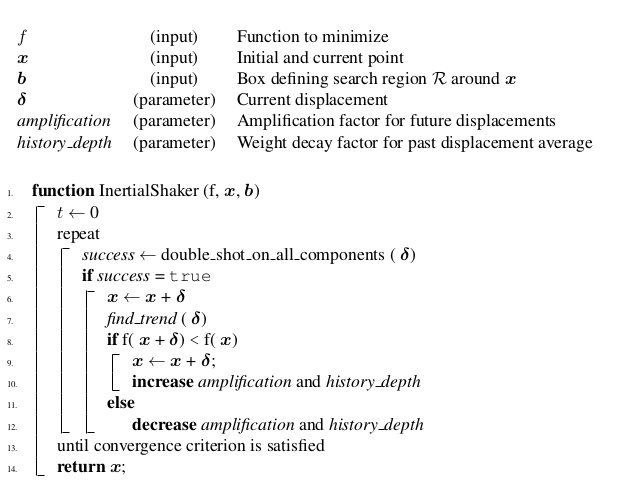
\includegraphics[scale=0.60]{is}
\caption{inertial shaker alg}
\centering
\end{figure}


\section{Derivative Based Optimization}

Derivative based optimization techniques help solving problems on continuous variables. We will focus on two major related problems:
\begin{itemize}
\item{Solving a set of non-linear equations \\
	\begin{itemize}
	\item{ $ \text{Given } F : {\rm I\!R}^n \rightarrow {\rm I\!R}^n $ }
	\item{ $ \text{Find } x^\ast \in {\rm I\!R}^n \text{ such that } F(x^\ast) = 0 \longrightarrow \text{ if } x^\ast \text{ exists it minimizes } \sum_{i=1}^{n} f_i(x)^2 = 0 $ }
	\end{itemize}
}\bigskip
\item{
	Unconstrained minimization \\
	\begin{itemize}
	\item{ $ f : {\rm I\!R}^n \rightarrow {\rm I\!R}^n $ }
	\item{ $ \text{Find } x^\ast \in {\rm I\!R}^n \text{ such that } f(x^\ast) \leq f(x) \ \forall x \in {\rm I\!R}^n \longrightarrow x^\ast \text{ if global minima } $ }
	\end{itemize}
}
\end{itemize}
This chapter will collect some techniques to optimize smooth (derivable) functions on continuous variables. A function is derivable in a if exists the limit $$
f'(a) = \lim_{h\to0} \frac{f(a+h) - f(a)}{h} $$ If $x$ is very close to the point of interest $a$ ($h = x-a$), we can approximate the function in $x$ with $$ f(a+h) \approx f(a) + f'(a)*h $$ Like skis are tools for descending slopes, derivatives are useful tools to build local model and to minimize the objective function iteratively.

\subsection{Optimization and machine learning}

There is a deep relation between Optimization and ML because each one is used by the other to improve performances. ``Optimization for Learning'' is the art of choosing best model and variables configurations to let our machine learning system perform better. An example is to choose the best combination of weights in a NN. On the other side ``Learning for Optimization'' is the science of using learning techniques to improve the search of global minima that depends on the past steps done by the algorithm. This allows to build algorithms that have a memory of what they already did, for example to avoid visiting a non-interesting attraction basin more than once.

\subsection{Derivative based techniques in one dimension}
We start with a historical and fundamental method to find the point where the function is equal to 0, starting from a sufficiently close point and repeating the following steps:
\begin{itemize}
\item{Find a solvable local model}
\item{Solve the local model}
\end{itemize}
The local model can be found with:
\begin{itemize}
\item{the Taylor series approximation: $ f(x) = f(x_{c}) + f'(x_{c}) (x - x_{c}) + \frac{f''(x_{c}) (x-x_{c})^2}{2!} + ...$ }
\item{or the Newton's theorem: $ f(x) = f(x_{c}) + \int_{x_{c}}^{x} f'(z) dz \approx f(x_{c}) + f'(x_{c}) (x - x_{c}) $ }
\end{itemize}
The local model is therefore $$ M_{c}(x) = f(x_{c}) + f'(x_{c}) (x - x_{c}) $$ and so the next value $x_{+}$ will be $$ x_{+} = x_{c} - \frac{f(x_{c})}{f'(x_{c})} $$ 
If the function is linear, convergence occurs in one step, on the other case, it is possible to prove that if one starts close enough the the local minima, it will reach it in a fast (quadratic) manner.
\par
A global and safe algorithm to find roots of a function is the bisection method: if the function is continuous and we know at least two point $l_{0}$ and $r_{0}$ such that $f(l_{0}) < 0$ and $f(r_{0}) > 0$, the bisection method converges in a logarithmic number of steps. The cons is that it works only in one dimension.
\par
An other idea is to use backtracking: if Newton steps leads too far, one reverts the direction returning closer to the root. Finally, what usually expert do is to combine some powerful local convergence method (like Newton's) with others that are global and robust.
\par
Derivatives are not always available but can be approximated with secants. One can use the value of the previous iteration $f(x_{-})$ to find an approximation of the inclination: $$ a_{c} = \frac{f(x_{c}) - f(x_{-})}{x_{c} - x_{-}} $$ Given the less accuracy, convergence will be slower. 

\subsection{Solving models in more than one dimension}
Newton's method requires the gradient to be equal to zero. Given step $s$, the quadratic model is: $$Q(s) = \sum_{i=1}^{n} g_{i} s_{i} + \sum_{i=1}^{n} \sum_{j=1}^{n} H_{ij} s_{i} s_{j} \equiv g^{T} s + \frac{1}{2} s^{T} H s$$ The quadratic model is an reduction of the Taylor series to the second order, trying to approximate the objective function with a parabola in $n$ dimensions. Like many other times, we are searching a point where the gradient equals 0: $$ \nabla Q(s) = 0 = g +Hs $$ $$ Hs^{n} = -g \text{ (Newton equation)} $$ Because of the limited precision of real number on computers, one has to deal with numerical stability, so the computed value can be slightly different from the real solution. Ill-Conditioning is a term used to measure how much a function is sensitive to some errors in the data. There are cases in which very small oscillations in the input values lead to big changes in the output value of f, and has to be avoided.

\subsubsection{Gradient or steepest descent}
Often one has to work with many many dimensions and quadratic forms becomes inefficient. Moreover the Hessian H matrix is not always available and even an approximation in difficult to be computed. The base form of gradient descent updates the actual $x$ value in this way: $$ x_{+} = x_{c} - \epsilon \nabla f $$ This method has no global view of the actual situation, only local informations are available. A frequent problem arise with ill-conditioned matrices: when the quadratic form is ill-conditioned, the gradient inherits the computational errors and does not precisely point toward the local minima. So, it's important to design algorithms that do not ``zigzag'' toward the local minima but that try to keep a pretty linear trajectory, reducing so the time needed to reach the bottom of the valley.

\subsection{Non linear Optimization in more Dimensions}
The extension of the Newton's method in more dimensions consists in solving the following model: $$ m_{c} (x_{c} + p) = f(x_{c}) + \nabla f(x_{c})^T p + \frac{1}{2} p^T \nabla^2 f(x_{c}) p $$ Basically, given that we know the value and the gradient of the function in $x_{c}$, it is possible to approximate the value in close points $(x_{c} + p)$. If the initial point is close enough to the minimizer $x^*$ and the matrix $\nabla^2 f(x_{c})$ is positive definite, the method converges Q-quadratically to $x^*$. (If the Hessian H or it's approximation $\nabla^2 f(x_{c})$ are not positive definite, the method is not guaranteed to converge because the gradient is not guaranteed to point to the local minima).

\subsubsection{Global Convergence through Line Searches}
Global convergence is obtained by adopting line searches along the identified direction: one tries Newton's method first and then possibly backtracks.

\subsubsection{Secant methods}
Useful when Hessian H matrix is not available or too costly to be calculated. Given two near points, second derivative can be obtained calculating the ``variation of the gradient''. Like derivatives are given by the amount of change of the function in a given step $x_{2} - x_{1}$, second derivatives can be seen as the variation of first derivatives in $x_{2} - x_{1}$ (one-dimensional example):
$$ \frac{d^2 f(x)}{d x^2} (x_{2} - x_{1}) \approx \bigg( \frac{df(x_{2})}{dx} - \frac{df(x_{1})}{dx} \bigg) $$
In more dimensions one equation is not sufficient. Let the current and next point be $x_{c}$ and $x_{+}$, respectively, and let's define $s_{c} = x_{+} - x_{c}$ and $y_{c} = \nabla f(x_{+}) - \nabla f(x_{c})$ (difference of gradients). The analogous ``secant equation'' is
$$
H_{+} s_{c} = y_{c}
$$
Given that this equation has $O(n^2)$ admissible solution, past history is often used to choose the best one.

\subsubsection{Closing the GAP: second-order methods with linear complexity}
Computing the exact Hessian matrix (the one that contains the coefficients of the second order derivatives or ``the gradient of the gradient'') requires $O(n^2)$ time and $O(n^2)$ memory, in addition to the $O(n^3)$ complexity of finding next step in Newton method. OSS (One-step-secant) uses the info about the last gradient to approximate the new H matrix in linear time $O(n)$ with the secant method.
The new search direction $p_{+}$ is computed as follow:
$$
p_{+} = -g_{c} + A_{c} s_{c} + B_{c} y_{c}
$$
with $A_{c}$ and $B_{c}$ that weights first and second derivatives.

\subsection{Constrained Optimization and Lagrange Multipliers}
This section will shows briefly hot to deal with contraints, that is, with some restrictions on the input (features) space. A general constrained minimization problem is: 
$$
\min_{x}		f(x)$$
$$\text{subject to }		(g_{i} (x) = c_{i}) \ \forall i = 1,...,n \ \ \text{(Equality Contraints)}$$
$$			(h_{j} \geq d_{j}) \ \forall j = 1,...,m \ \ \text{(Inequality Contraints)}$$

Contraints are divided in two categories:
\begin{itemize}
\item{Hard Contraints, that must be respected at all cost (very rare in practice)}
\item{Soft Contraints, that can be violated paying a penality}
\end{itemize}
Soft Constraints are more interesting; an example of penalized objective function is:
$$
\min_{x} f(x) + \sum_{i} \gamma_{i} (g_{i}(x) - c_{i})^2
$$
In this case, the penalties increase quadratically with the ``error'' $(g_{i}(x) - c_{i} )$. If the function is smooth (derivable) and has partial derivates, this type of problem are usually solved with Lagrange multipliers:

$$
\min_{x} f(x) + \sum_{i} \lambda_{i} g_{i}(x)
$$ 

Minimizing the transformed function yields a necessary condition for optimality. Additional checks are therefore necessary (for example, the identified point can be a saddle point and not a global minimum), but in many cases, in the presence of a single global optimum, the method of Lagrange multipliers will deliver the correct solution.





\end{document}

